\section{Bibliographie}

%-----------------------
\subsection{Bibliographie}

\begin{frame}[fragile]
  \frametitle{\insertsubsection}
  \begin{itemize}
    \item Avec \LaTeX{}, la bibliographie est séparée du reste dans un fichier \texttt{.bib} (par exemple: \texttt{biblio.bib}).
    \item L'utilisation d'une bibliographie requièrent les paquets suivants :
    \begin{itemize}
    \item \lstinline|\usepackage[backend=bibtex]{biblatex}|
    \item \lstinline|\usepackage{csquotes}|.
    \end{itemize}
    \item On utilise le fichier \texttt{biblio.bib} dans le document via la commande \lstinline|\bibliography{biblio.bib}| (dans l'en-tête du document).
    \item On cite un document avec la commande \lstinline|\cite{identifiant}|. Cet identifiant est repris dans le fichier \texttt{.bib}.
    \item On affiche la bibliographie à l'endroit souhaité avec la commande \lstinline|\printbibliography|.
  \end{itemize}
\end{frame}

\begin{frame}[fragile,allowframebreaks]
  \frametitle{Structure du fichier \texttt{.bib}}
  \begin{itemize}
      \item Pour chaque référence bibliographique, on ajoute une entrée au fichier. Exemple avec un article de Laurent Francis:
        \begin{lstlisting}[style=nonumbers]
  @inproceedings{ray2017challenges,
      title={Challenges of monolithic integration for SiGe MEMS technology},
      author={Ray Chaudhuri, Ashesh and Severi, S and Helin, P and Francis, Laurent and Tilmans, HAC},
      booktitle={15th IEEE Sensors Conference, SENSORS 2016},
      year={2017}
  }
        \end{lstlisting}
      Et un autre qui fit beaucoup de bruit:
      \begin{lstlisting}[style=nonumbers]
  @article{lemaitre1934evolution,
      title={Evolution of the expanding universe},
      author={Lema{\^\i}tre, Georges},
      journal={Proceedings of the National Academy of Sciences},
      volume={20}, number={1}, pages={12--17},
      year={1934},
      publisher={National Acad Sciences}
  }
      \end{lstlisting}
      \framebreak
      Et encore un autre, que nous ne citerons pas:
      \begin{lstlisting}[style=nonumbers]
  @article{de1966functions,
    title={Functions of lysosomes},
    author={De Duve, Christian and Wattiaux, Robert},
    journal={Annual review of physiology},
    year={1966},
    publisher={Annual Reviews 4139 El Camino Way, PO Box 10139, Palo Alto CA 94303-0139}
  }
      \end{lstlisting}
  \end{itemize}
\end{frame}

\begin{frame}[fragile]
  \frametitle{Exporter des \texttt{.bib}}
  \framesubtitle{Par exemple sur Google Scholar :}
  \begin{center}
  \includegraphics[width=\textwidth]{img/scholar.png}
  \end{center}
\end{frame}

\begin{frame}[fragile]
  \frametitle{Style de bibliographie}
  \begin{itemize}
      \item Le style est défini lors de l'appel du paquet \lstinline|\usepackage[style=ieee]{biblatex}|
      \item Les différents styles sont:
      \begin{itemize}
          \item \texttt{apa}, American Psychological Association;
          \item \texttt{chicago-authordate}, Chicago Style;
          \item \texttt{ieee}, Institute of Electrical and Electronics Engineers (IEEE).
      \end{itemize}
      \item Pour plus de style de bibliographie, voir \url{https://www.overleaf.com/learn/latex/Biblatex_citation_styles} et Google.
  \end{itemize}
\end{frame}

\begin{frame}[fragile]
  \frametitle{Exemple}
  \begin{columns}
    \begin{column}{0.5\textwidth}
      \begin{lstlisting}[style=nonumbers,mathescape]
      \documentclass[11pt]{scrartcl}
      \usepackage[utf8]{inputenc}
      \usepackage[T1]{fontenc}
      \usepackage[backend=bibtex]{biblatex}
      \usepackage{csquotes}
      \usepackage[french]{babel}
      \$\color{blue}{\texttt{bibliography\{monfichier.bib\}}}$
      \begin{document}
      Lorem ipsum dolor sit amet\$\color{blue}{\texttt{cite}}${delzottismartnic}, (...)
      Cras viverra\$\color{blue}{\texttt{cite}}${derdma} metus rhoncus sem. Nulla et lectus vestibulum
      urna fringilla ultrices.
      \$\color{blue}{\texttt{nocite}}${higginsonreal}
      \$\color{blue}{\texttt{printbibliography}}$
      \end{document}
          \end{lstlisting}
    \end{column}
    \begin{column}{0.5\textwidth}
      \centering
      \fbox{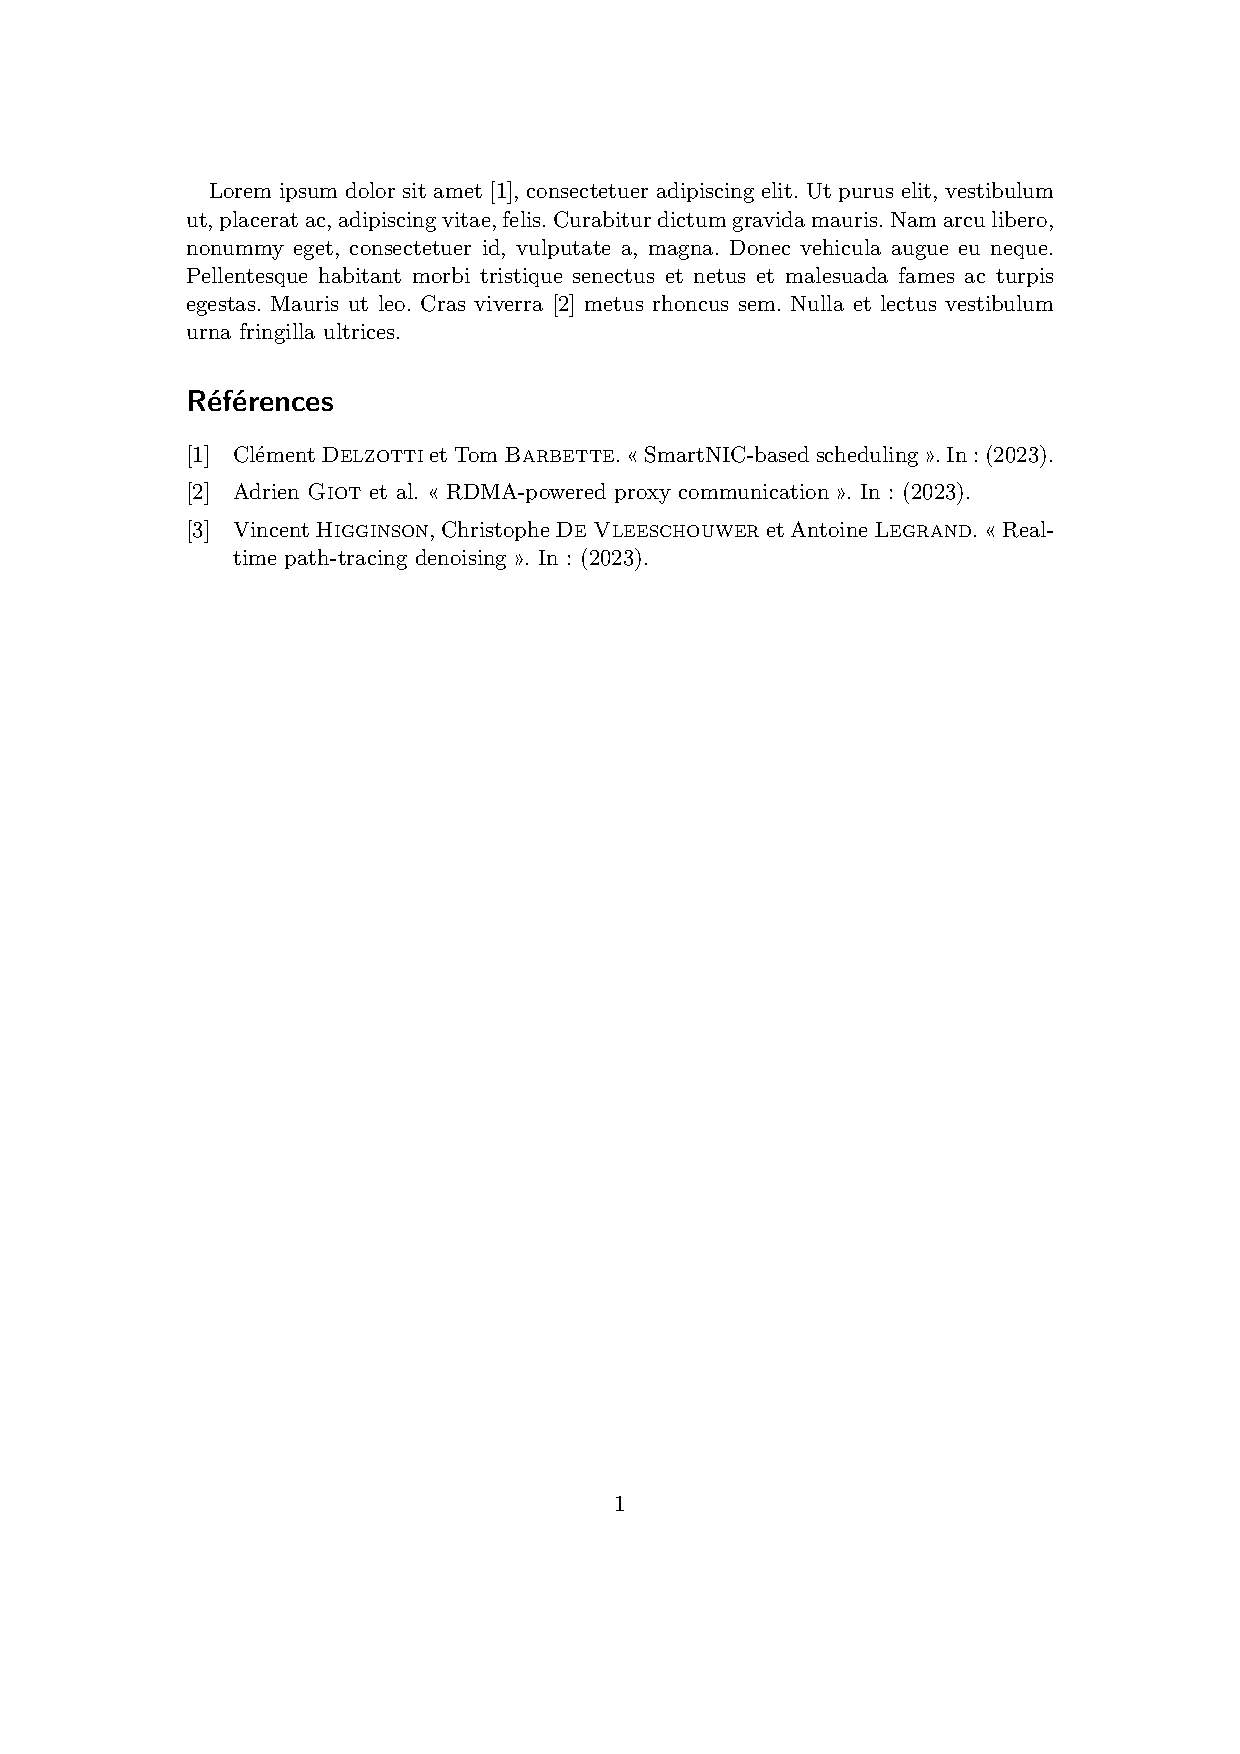
\includegraphics[width=1\textwidth,trim={1.5cm 10cm 1.5cm 1cm},clip]{../build_latex/examples/biblio/main.pdf}}
    \end{column}
  \end{columns}
  
  \begin{itemize}
      \item La commande \lstinline|\nocite{}| permet d'inclure dans la bibliographie un élément dans la bibliographie qui n'a pas été cité dans le texte.
  \end{itemize}
\end{frame}

\begin{frame}[fragile]
  \frametitle{\Warning Compilation}
  \begin{itemize}
      \item Pour \textbf{TeXMaker}
      \begin{itemize}
          \item Options $\rightarrow$ Configurer Texmaker $\rightarrow$ Compil rapide $\rightarrow$ Sélectionner ``PdfLaTex + BibLaTeX + PdfLaTeX (2x) + Voir pdf''
      \end{itemize}
      \item Pour \textbf{Overleaf}
      \begin{itemize}
          \item Fonctionne déjà dans la compilation de base.
      \end{itemize}
  \end{itemize}
\end{frame}

\begin{frame}[fragile]
  \frametitle{Troisième exercice}
  \begin{center}
      Compiler l'exemple de bibliographie et ajouter une référence depuis Google Scholar.\vspace{0.5cm}
      \fbox{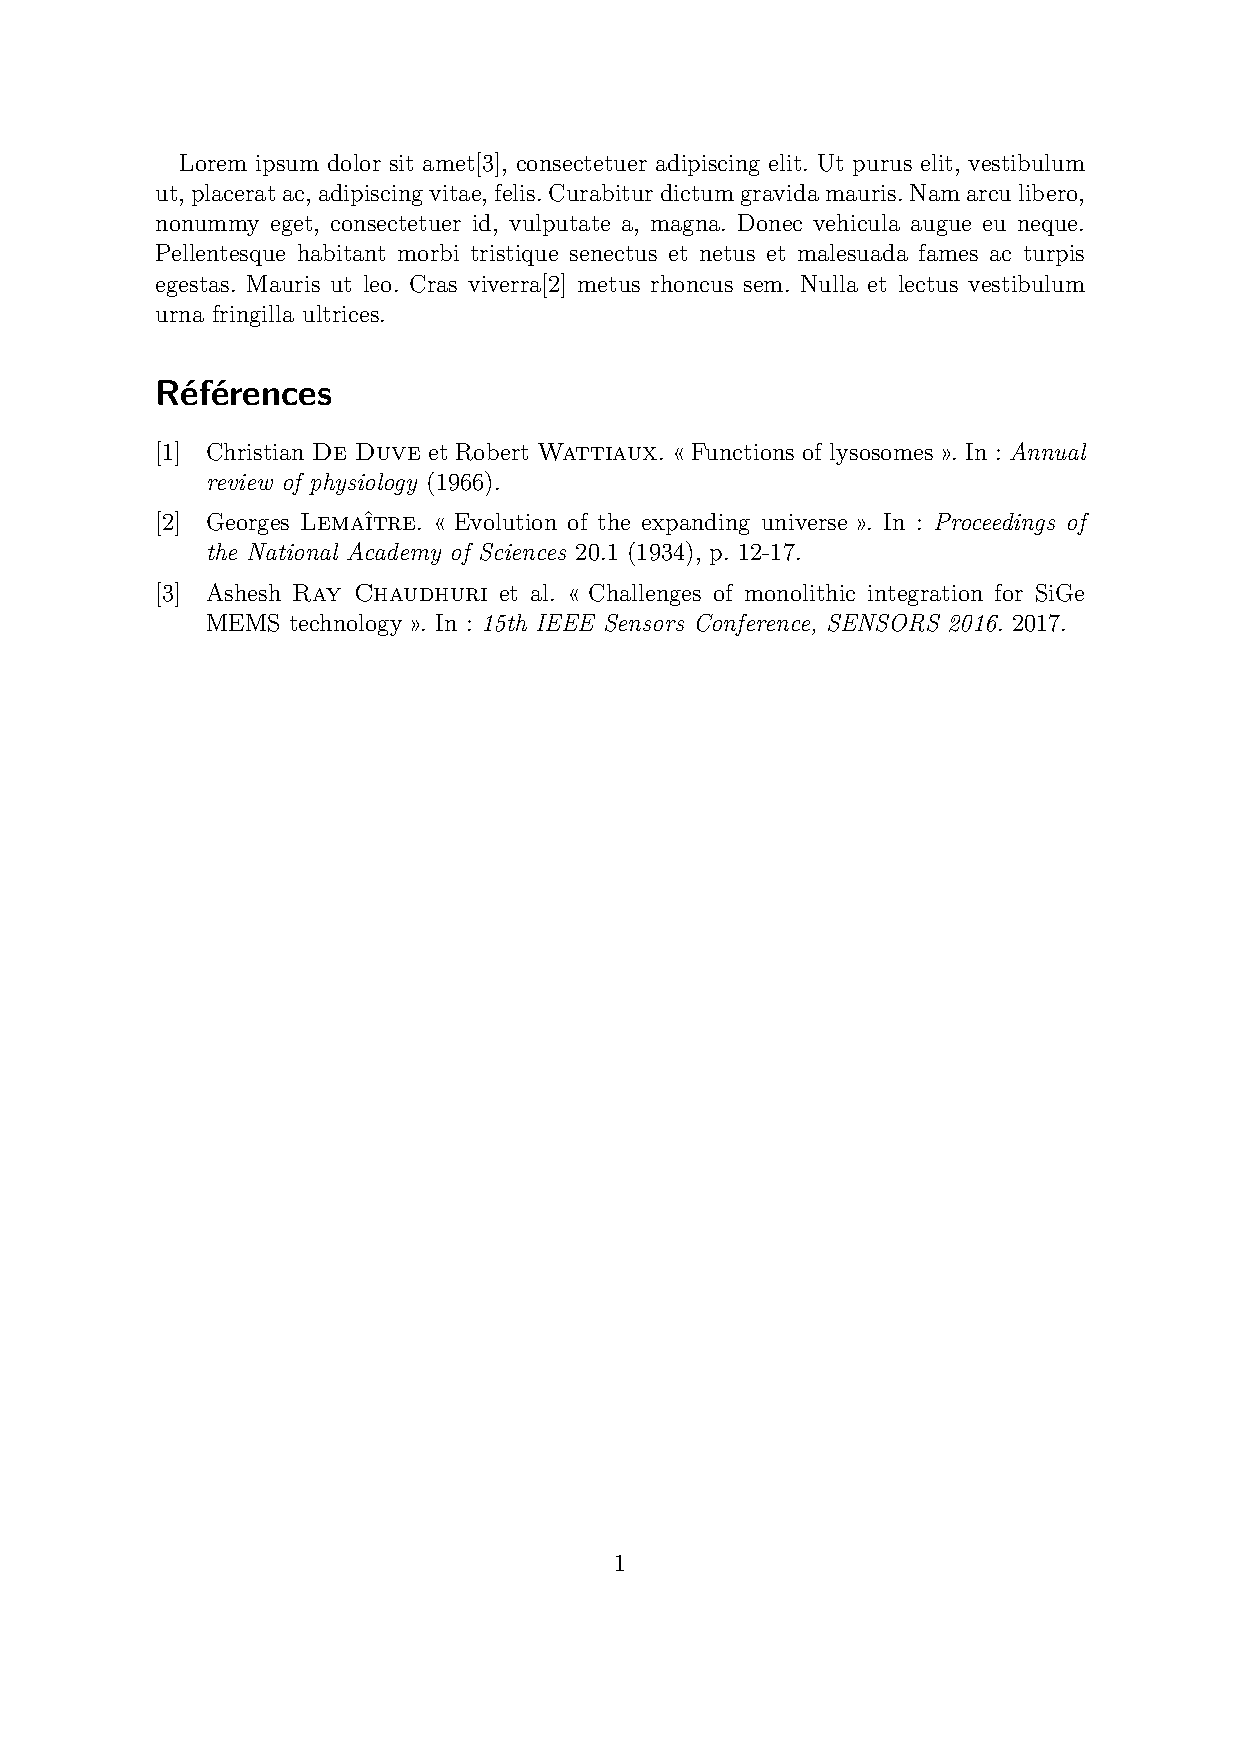
\includegraphics[width=0.8\textwidth,trim={2cm 18cm 2cm 2cm},clip]{../build_latex/exercices/bib/main.pdf}}
  \end{center}
\end{frame}

\begin{frame}[fragile]{Troisième exercice (solution)}
  \begin{center}
  Lien de la solution du troisième exercice \url{https://gitlab.com/louvainlinux/atelier-latex/-/raw/master/src/exercices/bib/main.tex}


  Lien du fichier bib : \url{https://gitlab.com/louvainlinux/atelier-latex/-/raw/master/src/exercices/bib/biblio.bib}
  \end{center}
\end{frame}

%-----------------------
\subsection{Découpe d'un projet en fichiers}

\begin{frame}[fragile]
  \frametitle{\Warning Découpe d'un projet en fichiers}
  \begin{itemize}
    \item Si vous travaillez sur un projet de moyenne ou grande envergure, il vaut la peine de le découper en plusieurs fichiers
    \item Cela accélère la recompilation et permet une séparation plus claire entre les sections
    \item Par exemple, un article pourrait avoir un fichier par section:
    \begin{itemize}
      \item \texttt{main.tex} contient la structure et l'en-tête du projet;
      \item \texttt{intro.tex} contient l'introduction et les remerciements;
      \item \texttt{section1.tex} contient la première section et son titre;
      \item \texttt{section2.tex} contient la deuxième section et son titre;
      \item \dots
    \end{itemize}
    \item L'inclusion dans fichier dans un autre se fait via la commande \lstinline|\input{}|.
  \end{itemize}
\end{frame}

\begin{comment}
\begin{frame}[fragile]
  \frametitle{Découpe d'un projet en fichiers}
  \framesubtitle{input et include}
  \begin{itemize}
    \item Deux commandes permettent l'inclusion d'un fichier dans un autre: \lstinline|\input{}| et \lstinline|\include{}|
    \item On leur donne en argument le nom du fichier sans le \texttt{.tex}
    \item \lstinline|\input{}| \og{}copie\fg{} le document littéralement
    \item \lstinline|\include{}| termine la page courante, copie le document, puis termine la page courante à nouveau
    \item \lstinline|\input{}| peut se trouver n'importe où, y compris dans le préambule, tandis que \lstinline|\include{}| doit se trouver dans le corps du document
    \item \lstinline|\include{}| accélère la compilation du document, car cela permet de ne recompiler que ce qui a été modifié
    \item La commande \lstinline|\includeonly{doc1,doc2,...}| permet de restreindre les documents à inclure
  \end{itemize}
\end{frame}
\end{comment}

\begin{frame}[fragile]
  \frametitle{\Warning Découpe d'un projet en fichiers}
  \framesubtitle{Exemple de l'article}
  \begin{columns}
      \begin{column}{0.5\textwidth}
          Dans \texttt{main.tex}
          \begin{lstlisting}[style=nonumbers, mathescape]
\documentclass[a4paper]{scrartcl}
\usepackage[utf8]{inputenc}
\usepackage[T1]{fontenc}
\usepackage[french]{babel}

\begin{document}
\maketitle
\tableofcontents

\input{intro.tex}
\input{$\color{black}{\texttt{section}}$1.tex}
\input{$\color{black}{\texttt{section}}$2.tex}
...
\end{document}
          \end{lstlisting}
      \end{column}
      \begin{column}{0.5\textwidth}
          Dans \texttt{intro.tex}
          \begin{lstlisting}[style=nonumbers]
\begin{center}
Je dédie cet article à mon chat.
Tu nous a quitté trop vite, Dragibus.
Repose en paix.
\end{center}
          \end{lstlisting}

          Dans \texttt{section1.tex}
          \begin{lstlisting}[style=nonumbers]
\section{Le Louvain-li-Nux}
Le Louvain-li-Nux est un kot à projet
de Louvain-la-Neuve.
...
          \end{lstlisting}

          Dans \texttt{section2.tex}
          \begin{lstlisting}[style=nonumbers]
\section{Le Kotangente}
Le Kotangente est kot ami du
Louvain-li-Nux.
...
          \end{lstlisting}
      \end{column}
  \end{columns}
\end{frame}
